\section{Particiones y conteo}

\subsection{Introducción}
\begin{figure}[t]
	\centering
	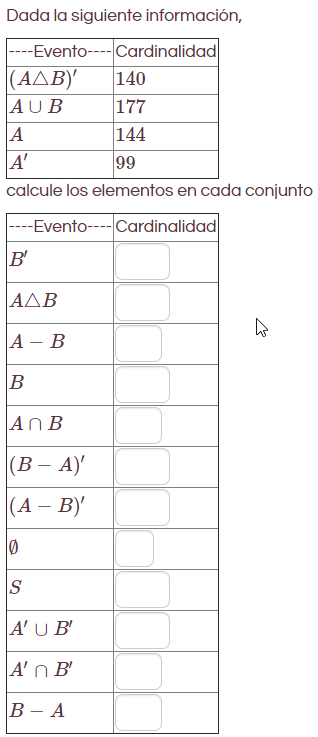
\includegraphics[height=250px]{./em/2020-08-15 19_49_02}
	\caption{Problema de conteo}
	\label{fig:problema-conteo}
\end{figure}[t]

En esta actividad resolveremos el problema planteado en la figura \ref{fig:problema-conteo}. Lo abordaremos con el siguiente plan:
\begin{enumerate}
	\item Definir una partición en un conjunto.
	\item Fijar una partición estándar para describir las operaciones entre dos conjuntos. 
	\item Describir las operaciones entre conjuntos utilizando esta partición.
	\item Plantear y resolver el problema en términos de dicha partición. 
\end{enumerate}


\subsection{Particiones}

Consideremos un conjunto $ S $. Una partición (finita) es una colección $ \set{P_i \subset S}_{i=0}^{N}, N \in \N $ de subconjuntos de $ S $ que satisface
\begin{enumerate}
	\item $ P_i \cap P_j =\emptyset $ siempre que $ i\neq j $;
	\item $ \bigcup_{i=0}^{N} P_i = S $. 
\end{enumerate}

En otras palabras, son subconjuntos disjuntos entre sí que, al unirse todos, forman de nuevo el conjunto $ S $. El lector puede pensarlos como piezas de un rompecabezas.

\begin{figure}[t]
	\centering
	
\includegraphics[width=0.7\linewidth]{./em/puzzle-5294291_1280}
	\caption[Rompecabezas]{Los rompecabezas son ejemplos de particiones.}
	\label{fig:puzzle-52942911280}
\end{figure}[t]

Consideremos dos conjuntos $ A,B \subset S$. El diagrama de Ven correspondiente esta dado por la figura \ref{fig:1280px-venndiagramforaunionb}. 

\begin{figure}[t]
	\centering
	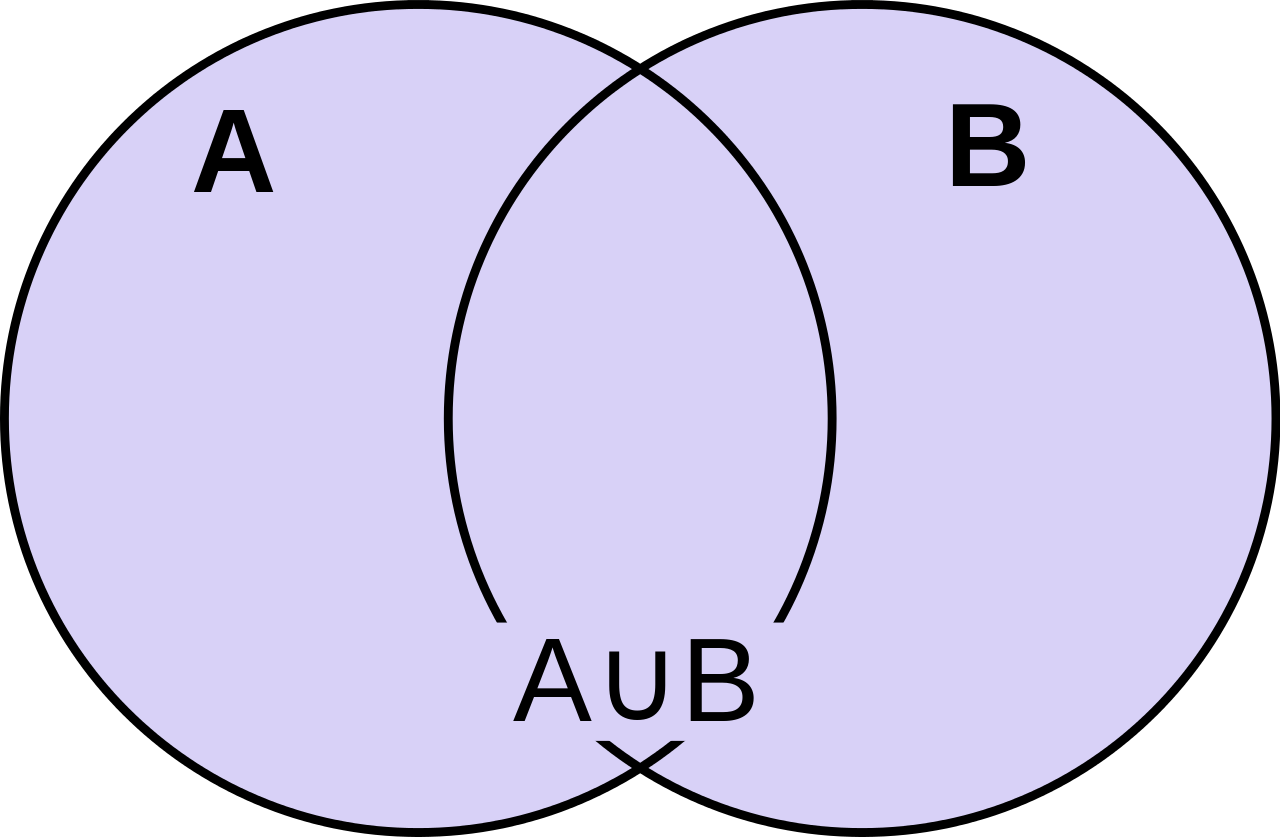
\includegraphics[width=0.7\linewidth]{./em/1280px-Venn_diagram_for_A_union_B.svg}
	\caption{Diagram de Ven para dos conjuntos}
	\label{fig:1280px-venndiagramforaunionb}
\end{figure}[t]

Entonces podemos definir una partición $ \particion(A,B) $ para $ S $ con los siguientes elementos
\begin{itemize}
	\item $ A\cap B $
	\item $ A\backslash B = A \cap B'$
	\item $ B\backslash A = B \cap A'$
	\item $ \left(A\cup B\right)' = A'\cap B' $
\end{itemize}

Para hacer la notación más concisa, definimos las siguientes aplicaciones:
\begin{align*}
	\delta_C(x) = \begin{cases}
		1 & x \in C \\
		0 & x \not \in C
	\end{cases}
\end{align*}
donde $ 1 $ denota \texttt{verdadero}, mientras que $ 0 $ denota \texttt{falso}, y
\begin{align*}
	E_{(i,j)}=\sett{x\in S}{\delta_{A}(x)=i\wedge\delta_{B}(x)=j}
\end{align*}
De manera que 
\begin{itemize}
	\item $ A' \cap B' = E_{(0,0)}$
	\item $ A'  \cap B = E_{(0,1)}$
	\item $ A \cap B'  = E_{(1,0)}$
	\item $ A  \cap B  = E_{(1,1)}$
\end{itemize}

Para hacer aún más sencilla la notación, identificaremos la pareja $ (i,j) $ con el correspondiente número binario $ [ij]_{2} $, convertido a base 10. De manera que 
\begin{itemize}
	\item $ A' \cap B' = E_{0}$
	\item $ A'  \cap B = E_{1}$
	\item $ A \cap B'  = E_{2}$
	\item $ A  \cap B  = E_{3}$
\end{itemize}

\subsection{Planteamiento del problema}

Como los elementos de un partición son disjuntos, entonces sabemos que 
\begin{align*}
	\#\left(E_i\cup E_j\right) = \#E_i+\#E_j
\end{align*}
siempre que $ i\neq j $.

Para simplificar la notación, definimos $ x_i=\# E_i. $

La primera ecuación que se nos plantea es
\begin{align*}
	\left(A \triangle B \right)'=140,
\end{align*}
donde 
\begin{align*}
	A\triangle B = (A\backslash B)\cup(B\backslash A)
\end{align*}
es la diferencia simétrica de $ A $ con $ B $. En otras palabras $ x\in A \triangle B $ si y solo si $ x\in A $ o $ x \in B $ pero no en ambos.

Observa que entonces
\begin{align}
	\label{ec01}
	\left(A\triangle B\right)' = E_0 \cup E_3 &
	\Rightarrow
	x_0 + x_3 = 140.
\end{align}

De manera similar, obtenemos las siguientes conclusiones:
\begin{align}
	\label{ec02}
	A\cup B = E_1\cup E_2 \cup E_3 &
	\Rightarrow x_1+x_2+x_3=177 \\
	\label{ec03}
	A = E_2 \cup E_3 &
	\Rightarrow x_2+x_3 = 144 \\
	\label{ec04}
	A' = E_0 \cup E_1 &
	\Rightarrow x_0+x_1 =99
\end{align}

Al resolver el sistema de ecuaciones dado por  \ref{ec01}-\ref{ec04}, obtenemos la solución:
\begin{align*}
	x_0 &= 66 \\
	x_1 &= 33 \\
	x_2 &= 70 \\
	x_3 &= 74
\end{align*}

\subsection{Solución del problema}

A continuación presentamos el desarrollo y conclusión de cada una de las preguntas en nuestro problema. Por ejemplo, podemos describir el complemento de $ B $ en términos de nuestra partición y utilizar las soluciones anteriores. 

\begin{align*}
	\# B' 
	&= \#\left(E_1 \cup E_3\right)'\\
	&= \#\left(E_0 \cup E_2\right)\\
	&= x_0 + x_2 = 153
\end{align*}

El resto de las soluciones se encuentras de la siguiente manera:

\begin{align*}
	\card{A\triangle B} = x_1+x_2 = 103  \\
	\card{A\backslash B} = x_2 = 70 \\
	\card{B} = x_1+x_3=107	\\
	\card{A \cap B} = x_3 = 74 \\
	\card{\left(B\backslash A\right)'} 
	= x_0+x_2+x_3 = 210 \\
	\card{\left(A\backslash B\right)'}
	= x_0+x_1+x3 = 173 \\
	\card{\emptyset} = 0 \\
	\card{S} = x_0+x_1+x_2+x_3 = 243 \\
	\card{A' \cap B'} = x_0 = 66\\
	\card{B\backslash A} = x_1 = 33
\end{align*}

Con esto concluimos nuestro ejercicio. 